% Adapted from the thesis chapter on fair repetitive interval scheduling.
\begin{figure}
    \centering
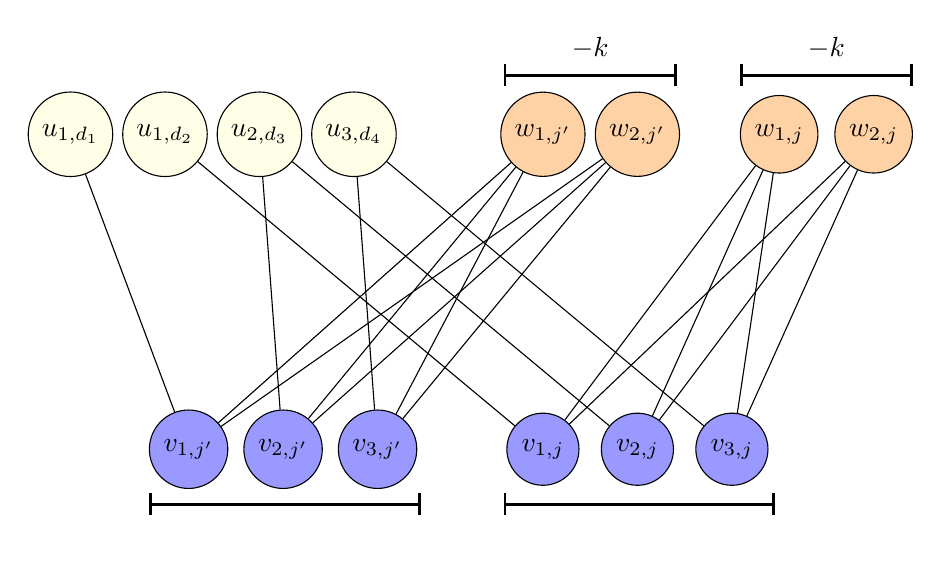
\begin{tikzpicture}

  \node[] at (1.2*1+3.5+1.75-4.5, -1.) {$\q$};
   \draw[line width=1, |-|]
  (1.2+3.5-4.5, -.7) -- (1.2*2+5.75-4.5, -.7) node[anchor=north] {};
  \foreach \i in {1,...,3} {
    \node[draw, circle, fill=blue!40] (A\i) at (\i*1.2-.5, 0) {$v_{\i,j'}$};
  }

  \node[] at (1.2*1+3.5+1.75, -1.) {$\q$};
   \draw[line width=1, |-|]
  (1.2+3.5, -.7) -- (1.2*2+5.75, -.7) node[anchor=north] {};
 
  \foreach \i in {1,...,3} {
    \node[draw, circle, fill=blue!40] (C\i) at (\i*1.2+4, 0) {$v_{\i,j}$};
  }
  
  \node[] at (1.2*1+4.6, 5.1) {$\q-k$};
   \draw[line width=1, |-|]
  (1.2+3.5, 4.75) -- (1.2*2+4.5, 4.75) node[anchor=north] {};
  \foreach \i in {1,...,2} {
    \node[draw, circle, fill=orange!35] (B\i) at (\i*1.2+4, 4) {$w_{\i,j'}$};
  }

  \node[] at (1.2*1+7.6, 5.1) {$\q-k$};
   \draw[line width=1, |-|]
  (1.2+6.5, 4.75) -- (1.2*2+7.5, 4.75) node[anchor=north] {};
  \foreach \i in {1,...,2} {
    \node[draw, circle, fill=orange!35] (D\i) at (\i*1.2+7, 4) {$w_{\i,j}$};
  }

    \node[draw, circle, fill=yellow!10] (F1) at (1*1.2-2, 4) {$u_{1,d_1}$};
    \node[draw, circle, fill=yellow!10] (F2) at (2*1.2-2, 4) {$u_{1,d_2}$};
    \node[draw, circle, fill=yellow!10] (F3) at (3*1.2-2, 4) {$u_{2,d_3}$};
    \node[draw, circle, fill=yellow!10] (F4) at (4*1.2-2, 4) {$u_{3,d_4}$};
                

  \foreach \i in {1,...,3} {
    \foreach \j in {1,...,2} {
      \draw (A\i) -- (B\j);
      \draw (C\i) -- (D\j);
    }
  }

    \draw (A1) -- (F1);
    \draw (C1) -- (F2);

    \draw (C2) -- (F3);
    \draw (A2) -- (F3);

    \draw (C3) -- (F4);
    \draw (A3) -- (F4);
    
\end{tikzpicture}

\caption{
The construction of a bipartite graph from an instance of \UEQUIJIT\ with $\q=3$ and $k=1$, where only the relevant vertices for two clients~$j$ and~$j'$ are depicted. Clients $j$ and~$j'$ have different due dates on day 1, and the same due date on days 2 and 3. Each client has two rejection vertices, adjacent to all three of that client's job vertices.}
\label{fig:bipartiteM}%
\end{figure}
